\documentclass[]{article}
\usepackage{lmodern}
\usepackage{amssymb,amsmath}
\usepackage{ifxetex,ifluatex}
\usepackage{fixltx2e} % provides \textsubscript
\ifnum 0\ifxetex 1\fi\ifluatex 1\fi=0 % if pdftex
  \usepackage[T1]{fontenc}
  \usepackage[utf8]{inputenc}
\else % if luatex or xelatex
  \ifxetex
    \usepackage{mathspec}
  \else
    \usepackage{fontspec}
  \fi
  \defaultfontfeatures{Ligatures=TeX,Scale=MatchLowercase}
\fi
% use upquote if available, for straight quotes in verbatim environments
\IfFileExists{upquote.sty}{\usepackage{upquote}}{}
% use microtype if available
\IfFileExists{microtype.sty}{%
\usepackage{microtype}
\UseMicrotypeSet[protrusion]{basicmath} % disable protrusion for tt fonts
}{}
\usepackage[margin=1in]{geometry}
\usepackage{hyperref}
\hypersetup{unicode=true,
            pdftitle={A DFT study to charactirized a suitable SiO2 messoporius support surface},
            pdfauthor={Ciellie Jansen van Vuuren},
            pdfborder={0 0 0},
            breaklinks=true}
\urlstyle{same}  % don't use monospace font for urls
\usepackage{graphicx,grffile}
\makeatletter
\def\maxwidth{\ifdim\Gin@nat@width>\linewidth\linewidth\else\Gin@nat@width\fi}
\def\maxheight{\ifdim\Gin@nat@height>\textheight\textheight\else\Gin@nat@height\fi}
\makeatother
% Scale images if necessary, so that they will not overflow the page
% margins by default, and it is still possible to overwrite the defaults
% using explicit options in \includegraphics[width, height, ...]{}
\setkeys{Gin}{width=\maxwidth,height=\maxheight,keepaspectratio}
\IfFileExists{parskip.sty}{%
\usepackage{parskip}
}{% else
\setlength{\parindent}{0pt}
\setlength{\parskip}{6pt plus 2pt minus 1pt}
}
\setlength{\emergencystretch}{3em}  % prevent overfull lines
\providecommand{\tightlist}{%
  \setlength{\itemsep}{0pt}\setlength{\parskip}{0pt}}
\setcounter{secnumdepth}{0}
% Redefines (sub)paragraphs to behave more like sections
\ifx\paragraph\undefined\else
\let\oldparagraph\paragraph
\renewcommand{\paragraph}[1]{\oldparagraph{#1}\mbox{}}
\fi
\ifx\subparagraph\undefined\else
\let\oldsubparagraph\subparagraph
\renewcommand{\subparagraph}[1]{\oldsubparagraph{#1}\mbox{}}
\fi

%%% Use protect on footnotes to avoid problems with footnotes in titles
\let\rmarkdownfootnote\footnote%
\def\footnote{\protect\rmarkdownfootnote}

%%% Change title format to be more compact
\usepackage{titling}

% Create subtitle command for use in maketitle
\newcommand{\subtitle}[1]{
  \posttitle{
    \begin{center}\large#1\end{center}
    }
}

\setlength{\droptitle}{-2em}
  \title{A DFT study to charactirized a suitable SiO\textsubscript{2} messoporius
support surface}
  \pretitle{\vspace{\droptitle}\centering\huge}
  \posttitle{\par}
  \author{Ciellie Jansen van Vuuren}
  \preauthor{\centering\large\emph}
  \postauthor{\par}
  \predate{\centering\large\emph}
  \postdate{\par}
  \date{09/03/2018}

\usepackage{ragged2e}
\usepackage{placeins}

\begin{document}
\maketitle

\hypertarget{section}{%
\subparagraph{}\label{section}}

\hypertarget{abstract}{%
\section{Abstract}\label{abstract}}

Three \(\alpha\)-Quartz ,spacegroup 180, surfaces were modelled using
crystallographic data from pearson\ldots{}. obtained in the Medea
package database. Surface planes with miller indexes 100, 110 and 200
were cut from the bulk structure. The different surfaces were compared
to identify the ideal MCM-41 surface to be used as a catalyst support.

\hypertarget{introduction}{%
\section{Introduction}\label{introduction}}

The utilisation of homogeneos catalysts in industry are limited, due to
the fact that it is expensive to extract the catalyst from post-reaction
mixtures (Balcar \& Čejka, 2013), (Kotzé, 2015). Research especialy in
the pharmaseutlical and petrochemistry industries took an intrest in the
imobilisation or heteroganasion of a homgeneous catalyst as a posible
solution to the mentiond problem.

Although the activity and selectivity of heterogeneous catalytic
reactions are lower than homogeneous reactions, the advantage of
separation, recovery and recycling outweigh these shortcomings. It is
however important to ensure that the effectiveness of the immobilized
homogeneous catalyst is not dramatically compromised (Kotzé, 2015),
(Gryp \emph{et al.}, 2010). Therefore the main objective in the
successful immobilization of homogeneous catalyst systems is to combine
the high activity and selectivity properties of homogeneous catalysts
with the ease of recovery of a heterogeneous catalyst. To accomplish
this the selection of an appropriate support material is very important
(Kotzé, 2015).

Support materials can be divided into three categories e.g.~insoluble
organic, polymeric or inorganic supports. Immobilization by using
insoluble organic supports involves ultrafiltration techniques as seen
in the separation of the PUK-Grubbs 2 catalyst by using organic solvent
nanofiltration (Gryp \emph{et al.}, 2010). Van der Gryp et al. (Gryp
\emph{et al.}, 2010) performed this separation using organic membranes
and discovered that the catalyst can be successfully separated, but its
lifetime was dramatically decreased during the filtration process (Gryp
\emph{et al.}, 2010), (Kotzé, 2015). Polymer supports on the other hand
provide easier filtration techniques, multiple coordination sites and
the possibility to incorporate a molecular catalyst into the polymer
structure. These are great advantages, but during the filtration process
the thermal stability remains low (Kotzé, 2015). Inorganic supports have
a high thermal stability, it provides for multiple coordination sites
because it contains a large surface area (BET), big pores and narrow
pore size distributions. Therefore inorganic supports are more effective
in the immobilization of homogeneous catalysts systems than organic or
polymeric support surfaces.(Balcar \& Čejka, 2013)

There are three types of inorganic supports available, which is
categorized by their pore sizes and physical compositions:

\begin{enumerate}
\def\labelenumi{\arabic{enumi}.}
\tightlist
\item
  Inorganic microporous support materials have pore sizes \textless{}
  2nm, e.g.~Zeolites, Metal-Organic Frameworks (MOFs);
\item
  Inorganic mesoporous support materials have pore sizes in the range of
  2-15 nm, e.g.~MCM-41, SBA-15 and Aerogels; and
\item
  Inorganic macroporous support materials have pore sizes greater than
  50 nm, e.g.~glasses. (Balcar \& Čejka, 2013), (Kotzé, 2015)
\end{enumerate}

Although microporous and macroporious support materials have the ability
to be used as heterogeneous support, it doesn't have an industrial
appeal yet (Balcar \& Čejka, 2013),(Kotzé, 2015). Therefore the focus is
on mesoporous support materials. Since the successful synthesis of
mesoporous materials by Mobil in 1992, the research field in using and
synthesizing mesoporious materials as support materials for
heterogeneous catalytic reactions has grown significantly. The original
synthesis of mesoporous support material was defined as the M41S family
containing hexagonal MCM-41, cubic MCM-48 and lamellar MCM-50
structures. A more visual representation of the different structures can
be seen in Figure 1

\begin{center}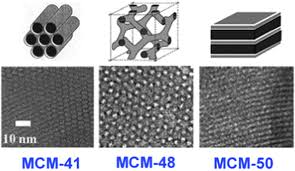
\includegraphics[width=0.9\linewidth]{Data/Images/Mcm-structures} \end{center}

Figure 1: Different structures of the M41S family (Linares \emph{et
al.}, 2014)

Unfortunately M41S materials have a limitation in pore diameter,
approximately 80 Å, which affects the separation of large molecules
(Katiyar \emph{et al.}, 2006). Zhao et al. (Zhao \emph{et al.}, 1998)
extended the family of inorganic mesoporous support materials by
synthesizing Santa Barbara Amorphous (SBA) type materials, with a pore
diameter ranging between 20 to 300 Å.

\hypertarget{surface-characterization}{%
\subsection{Surface characterization}\label{surface-characterization}}

The surface of mesoporous support materials are amporphious and contain
accessible hydroxyl groups. This makes immobilization of homogeneous
complexes on the silica surface possible (Kotzé, 2015). The crusial
factor for immobilization of a catalyst on the silica surface is the
concentration, distribution and accessibility of the silanol groups on
the silica surface (Balcar \& Čejka, 2013). Ramírez et al. (A. Ramı'rez
\& Sierra*, 2003) showed that the types of silanols present on the
silica surface are single, hydrogen bonded or germinal silanol groups as
shown in Figure 2.

Figure 2: Different silanol groups on the surface of a silica support:
(a) single, (b) hydrogen bonded and (c) geminal silanol groups {[}A.
Ramı'rez \& Sierra* (2003){]}

\begin{center}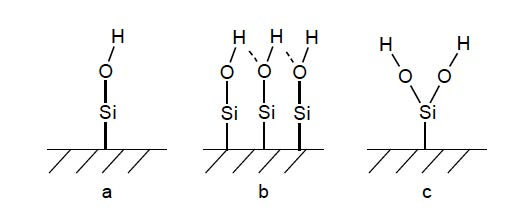
\includegraphics[width=7.11in]{Data/Images/Silanol_groups} \end{center}

Coordination of the metal complexes to the support can either take place
by binding of the metal ions directly or via organic molecule linkers to
the silanols. Sels and co-workers (Van Berlo \emph{et al.}, 2008)
observed that a weak physical interaction between a neutral
Hoveyda-Grubbs- II type complex and the inorganic support was enough to
seperate the complex from the mixture and altered surfaces using linkers
was not nessesary. Cabrera et al. (Cabrera \emph{et al.}, 2012) and
Schachner et al. (Schachner \emph{et al.}, 2011) also found that
ruthenium-based metathesis catalysts containing a hemilabile
pyridine-alkoxide ligand adsorb extremely well onto an unmodified silica
support without compromising too much on the homogeneous catalytic
effectiveness.

\hypertarget{experimental}{%
\section{Experimental}\label{experimental}}

\hypertarget{results-and-discussion}{%
\section{Results and discussion}\label{results-and-discussion}}

\listoffigures

\hypertarget{refs}{}
\leavevmode\hypertarget{ref-RN75}{}%
A. Ramı'rez, B. L. Lopez \& Sierra*, L. 2003. Study of the acidic sites
and their modifications in mesoporous silica synthesized in acidic
medium under quiescent conditions. \emph{Journal of Physical Chemistry}.
(107):5.

\leavevmode\hypertarget{ref-RN44}{}%
Balcar, H. \& Čejka, J. 2013. Mesoporous molecular sieves as advanced
supports for olefin metathesis catalysts. \emph{Coordination Chemistry
Reviews}. 257(21-22):3107--3124.

\leavevmode\hypertarget{ref-RN84}{}%
Cabrera, J., Padilla, R., Bru, M., Lindner, R., Kageyama, T., Wilckens,
K., Balof, S.L., Schanz, H.J., Dehn, R., Teles, J.H., Deuerlein, S.,
Muller, K., Rominger, F., \& Limbach, M. 2012. Linker-free, silica-bound
olefin-metathesis catalysts: Applications in heterogeneous catalysis.
\emph{Chemistry}. 18(46):14717--24.

\leavevmode\hypertarget{ref-RN73}{}%
Gryp, P. van der, Barnard, A., Cronje, J.-P., Vlieger, D. de, Marx, S.,
\& Vosloo, H.C.M. 2010. Separation of different metathesis grubbs-type
catalysts using organic solvent nanofiltration. \emph{Journal of
Membrane Science}. 353(1-2):70--77.

\leavevmode\hypertarget{ref-RN89}{}%
Katiyar, A., Yadav, S., Smirniotis, P.G., \& Pinto, N.G. 2006. Synthesis
of ordered large pore sba-15 spherical particles for adsorption of
biomolecules. \emph{J Chromatogr A}. 1122(1-2):13--20.

\leavevmode\hypertarget{ref-RN90}{}%
Kotzé, H. de V. 2015. Immobilized ru(II) catalysts for transfer
hydrogenation and oxidative alkene cleavage reactions (Journal Article).
Stellenbosh University South Africa.

\leavevmode\hypertarget{ref-RN87}{}%
Linares, N., Silvestre-Albero, A.M., Serrano, E., Silvestre-Albero, J.,
\& Garcia-Martinez, J. 2014. Mesoporous materials for clean energy
technologies. \emph{Chem Soc Rev}. 43(22):7681--717.

\leavevmode\hypertarget{ref-RN85}{}%
Schachner, J.A., Cabrera, J., Padilla, R., Fischer, C., Schaaf, P.A. van
der, Pretot, R., Rominger, F., \& Limbach, M. 2011. A set of olefin
metathesis catalysts with extraordinary stickiness to silica. \emph{ACS
Catalysis}. 1(8):872--876.

\leavevmode\hypertarget{ref-RN74}{}%
Van Berlo, B., Houthoofd, K., Sels, B., \& Jacobs, P. 2008. Silica
immobilized second generation hoveyda-grubbs: A convenient, recyclable
and storageable heterogeneous solid catalyst. \emph{Advanced Synthesis
\& Catalysis}. 350(13):1949--1953.

\leavevmode\hypertarget{ref-RN69}{}%
Zhao, D., Feng, J., Huo, Q., Melosh, N., Fredrickson, G.H., Chmelka,
B.F., \& Stucky, G.D. 1998. Triblock copolymer syntheses of mesoporous
silica with periodic 50 to 300 angstrom pores. \emph{SCIENCE}. 279(548).


\end{document}
